\section{Minimização de $||\VECTOR{f}(\VECTOR{x})-\VECTOR{b}||_{\MATRIX{C}}^2$}

%\index{Minimização, métodos!Regularização de }
%\index{Problema inverso!Não linear}
\index{Minimização do erro quadrático!Não linear}%!Função $||\VECTOR{f}(\VECTOR{x})-\VECTOR{b}||_{\MATRIX{C}}^2$}

\begin{theorem}[Solução iterativa]\label{theo:minfxbCfxb}
Dados,
os vetores coluna $\VECTOR{x}\in \mathbb{R}^N$ e $\VECTOR{b}\in \mathbb{R}^M$,  
uma função $\VECTOR{f}:\mathbb{R}^{N} \rightarrow \mathbb{R}^{M}$, 
uma matriz diagonal $\MATRIX{C} \in \mathbb{R}^{M\times M}_{+}$, e 
definida a Eq. (\ref{eq:minfxbCfxb1}),
\begin{equation}\label{eq:minfxbCfxb1}
\begin{matrix}
e(\VECTOR{x}) & = & ||\VECTOR{f}(\VECTOR{x})-\VECTOR{b}||_{\MATRIX{C}}^2 \\
              & = & (\VECTOR{f}(\VECTOR{x})-\VECTOR{b})^{\transpose}\MATRIX{C}(\VECTOR{f}(\VECTOR{x})-\VECTOR{b}).
\end{matrix}
\end{equation}
Se desejamos ter o ponto $\VECTOR{x}=\VECTOR{\hat{x}}$ que minimiza o escalar $e(\VECTOR{x})$,
podemos achar este ponto usando iterativamente a Eq. (\ref{eq:minfxbCfxb2}),
onde  $\MATRIX{J}(\VECTOR{x})$ é a \hyperref[def:jacobian]{\textbf{matriz Jacobiana}}  de $\VECTOR{f}(\VECTOR{x})$.
\begin{equation}\label{eq:minfxbCfxb2}
\VECTOR{x}_{k} \leftarrow \VECTOR{x}_{k-1}-
\left[ \MATRIX{J}(\VECTOR{x}_{k-1})^{\transpose}\MATRIX{C} \MATRIX{J}(\VECTOR{x}_{k-1}) \right]^{-1}
 \MATRIX{J}(\VECTOR{x}_{k-1})^{\transpose}\MATRIX{C}\left[\VECTOR{f}(\VECTOR{x}_{k-1})-\VECTOR{b}\right];
\end{equation}



Assim, $\VECTOR{\hat{x}}$ pode ser achado 
iniciando a Eq. (\ref{eq:minfxbCfxb2}) desde um $\VECTOR{x}_{0}$ qualquer, 
ate que $\VECTOR{x}_{k}$ seja muito próximo a $\VECTOR{x}_{k-1}$,
onde se declara que $\VECTOR{\hat{x}} \approx \VECTOR{x}_{k}$,
que corresponde a um mínimo\footnote{\label{ref:minfx}A
demostração pode ser vista na Prova \ref{proof:theo:minfxbCfxb}.} de $e(\VECTOR{x})$,
sem aclarar se é local ou global.

\textbf{Considerações:}

\begin{itemize}
\item Para que tenha sentido a Eq. (\ref{eq:minfxbCfxb2}),
 e consequentemente esta possa ser usada, devemos verificar que  $\MATRIX{J}(\VECTOR{x}_{k-1})\neq \MATRIX{0}$,
pois se $\MATRIX{J}(\VECTOR{x}_{k-1})= \MATRIX{0}$ indica que existe\footref{ref:minfx} um ponto de inflexão 
(máximo, mínimo ou ponto de sela) em $e(\VECTOR{x}_{k-1})$.
\item A busca iterativa da Eq. (\ref{eq:minfxbCfxb2}) é considerada falida quando 
$\MATRIX{J}(\VECTOR{x}_{k-1})^{\transpose}$ $\MATRIX{C}$ $\MATRIX{J}(\VECTOR{x}_{k-1})$
não tem inversa.
\item A busca iterativa da Eq. (\ref{eq:minfxbCfxb2}) pode diverger quando coincide que o mínimo $\VECTOR{\hat{x}}$ procurado
tem um $\MATRIX{J}(\VECTOR{\hat{x}})\approx \MATRIX{0}$.
O erro só acontece quando $\VECTOR{x}_{k-1}$ atinge de forma ``exata'' um mínimo com $\VECTOR{f}(\VECTOR{x}_{k-1})\neq \VECTOR{b}$,
para outros valores a busca iterativa de $\VECTOR{x}_{k-1}$ avança eficazmente.
\end{itemize}

\end{theorem}
%%%%%%%%%%%%%%%%%%%%%%%%%%%%%%%%%%%%%%%%%%%%%%%%%%%%%%%%%%%%%%%%%%%%%%%%%%%%%%%%
\subsection{Exemplos de minimização de $||\VECTOR{f}(\VECTOR{x})-\VECTOR{b}||_{\MATRIX{C}}^2$}

\begin{example}[Quando existe 
$\VECTOR{\hat{x}}$ que cumpre que $\VECTOR{f}(\VECTOR{\hat{x}}) \approx \VECTOR{b}$:]
\label{ex:minfxbCfxb}
Conhecida uma função $\VECTOR{f}(\VECTOR{x}) : \mathbb{R}^{2} \rightarrow \mathbb{R}^{3}$
é um ponto $\VECTOR{b}$ do contradominio de $\VECTOR{f}(\VECTOR{x})$,
achar o valor $\VECTOR{\hat{x}}$ que minimize $||\VECTOR{f}(\VECTOR{x})-\VECTOR{b}||_{\MATRIX{C}}^2$;
sabendo que:
\begin{equation}
\VECTOR{b}=\begin{bmatrix}
1\\
1\\
2
\end{bmatrix},
\qquad 
\VECTOR{f}(\VECTOR{x})=\begin{bmatrix}
x_1^2\\
x_2^2\\
x_1+x_2
\end{bmatrix}.
\end{equation}
Consequentemente podemos deduzir e escolher que, 
\begin{equation}\label{eq:lab:ex2fx}
\MATRIX{J}(\VECTOR{x})=\begin{bmatrix}
2 x_1 & 0\\
0 & 2 x_2\\
1 & 1
\end{bmatrix},
\qquad
\MATRIX{C}=\begin{bmatrix}
1 & 0 & 0\\
0 & 1 & 0\\
0 & 0 & 1
\end{bmatrix}.
\end{equation}
Com todos estes dados e usando a Eq. (\ref{eq:minfxbCfxb1}),
obtemos a superfície $e(\VECTOR{x})$ como mostra a Figura \ref{fig:ex:minfxbCfxb:a}.
Podemos ver as respostas a este exemplo na Solução \ref{ex:minfxbCfxb:sol1} e \ref{ex:minfxbCfxb:sol2}.
\end{example}

\begin{SolutionT}[Relativa ao Exemplo \ref{ex:minfxbCfxb}:]
\label{ex:minfxbCfxb:sol1}
Se escolhemos o ponto inicial $\VECTOR{x}_0=[0.1~0.1]^{\transpose}$ e 
usamos iterativamente a Eq. (\ref{eq:minfxbCfxb2}), obtemos os valores 
de $\VECTOR{x}_k$ e $e(\VECTOR{x}_k)$, como mostra a Tabela \ref{table:ex:minfxbCfxb},
onde se asume o final do processo iterativo quando $\VECTOR{x}_k \approx \VECTOR{x}_{k-1}$.
Assim, a aproximação iterativa conclui na resposta $\VECTOR{\hat{x}}\approx \VECTOR{x}_{4} =[1~1]^{\transpose}$,
com um erro $e(\VECTOR{\hat{x}})=5.0032~10^{-24}\approx 0$ e uma pendente\footnote{\label{ref:pendenteex} O
cálculo da pendente de $e(\VECTOR{\hat{x}})$ pode ser vista no Teorema \ref{theo:derfxbCfxb0}.}
$\frac{\partial e(\VECTOR{\hat{x}})}{\partial \VECTOR{x} }=[7.7485~10^{-12}\quad 7.7485~10^{-12}]^{\transpose}$
próxima a zero;
este processo pode ser visto de forma gráfica na Figura \ref{fig:ex:minfxbCfxb:b}.
\end{SolutionT}


\begin{table}[h!]
\centering
\begin{tabular}{|l|l|l|l|l|l|}
\hline
$k$ & 0 & 1 & 2 & 3 & 4 \\ \hline
$\VECTOR{x}_k$ & 0.10000   & 1.07941   & 1.00204   & 1.00000   & 1.00000 \\ 
~              & 0.10000   & 1.07941   & 1.00204   & 1.00000   & 1.00000 \\ \hline
$||\VECTOR{x}_k||$ & 0.14142   & 1.52652   & 1.41710   & 1.41421   & 1.41421 \\ \hline
$e(\VECTOR{x}_k)$ & 5.2002 &   7.9761e-02  & 5.0203e-05  & 2.3241e-11  & 5.0032e-24 \\ \hline
\end{tabular}
\caption{Resposta iterativa do Exemplo \ref{ex:minfxbCfxb}.}
\label{table:ex:minfxbCfxb}
\end{table}
\begin{figure}[h!]
     \centering
     \begin{subfigure}[b]{0.49\textwidth}
         \centering
         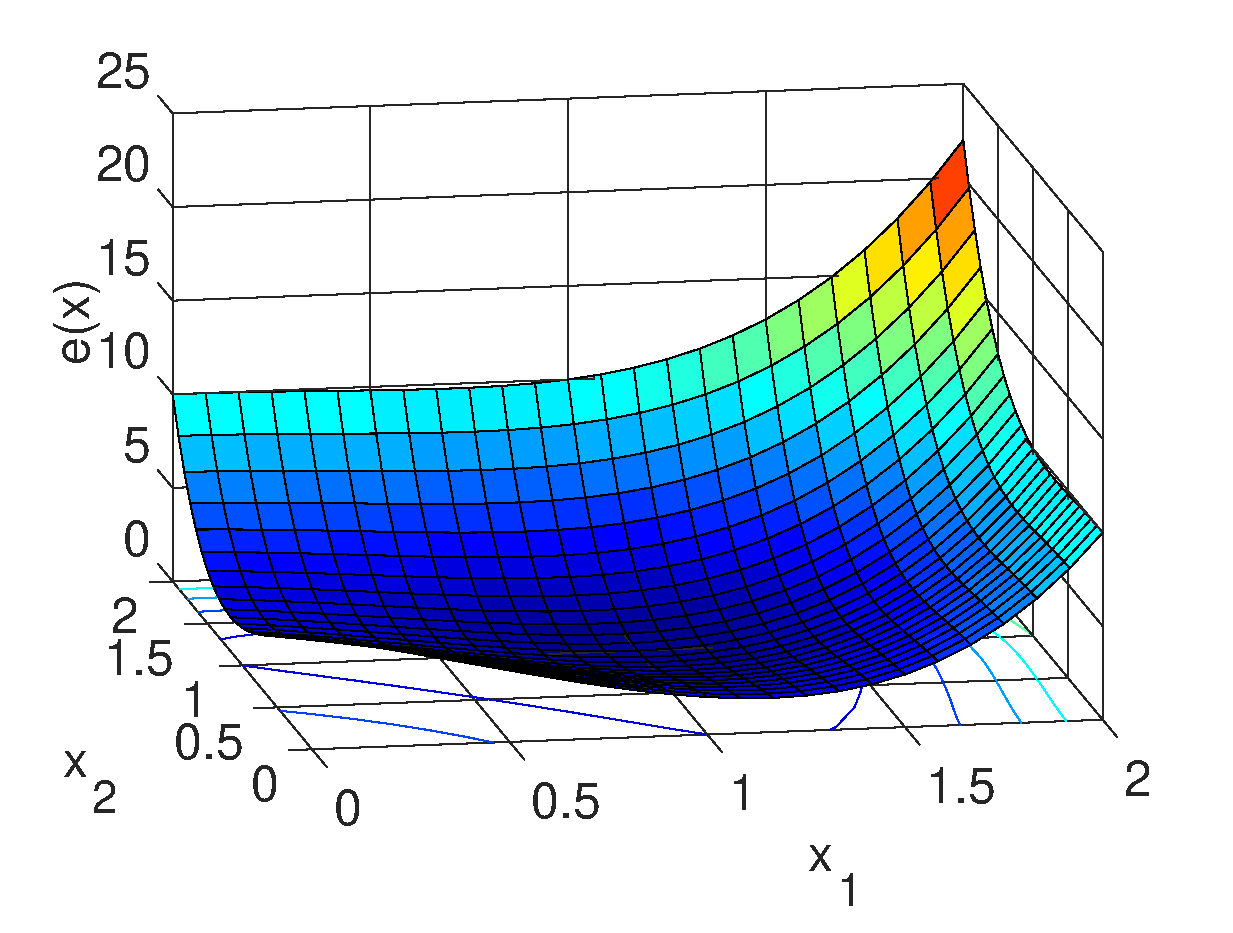
\includegraphics[width=0.98\textwidth]{chapters/minimization-fx/mfiles/fx1/surfcfx.eps}
         \caption{Superfície $e(\VECTOR{x})$. }
         \label{fig:ex:minfxbCfxb:a}
     \end{subfigure}
     \hfill
     \begin{subfigure}[b]{0.49\textwidth}
         \centering
         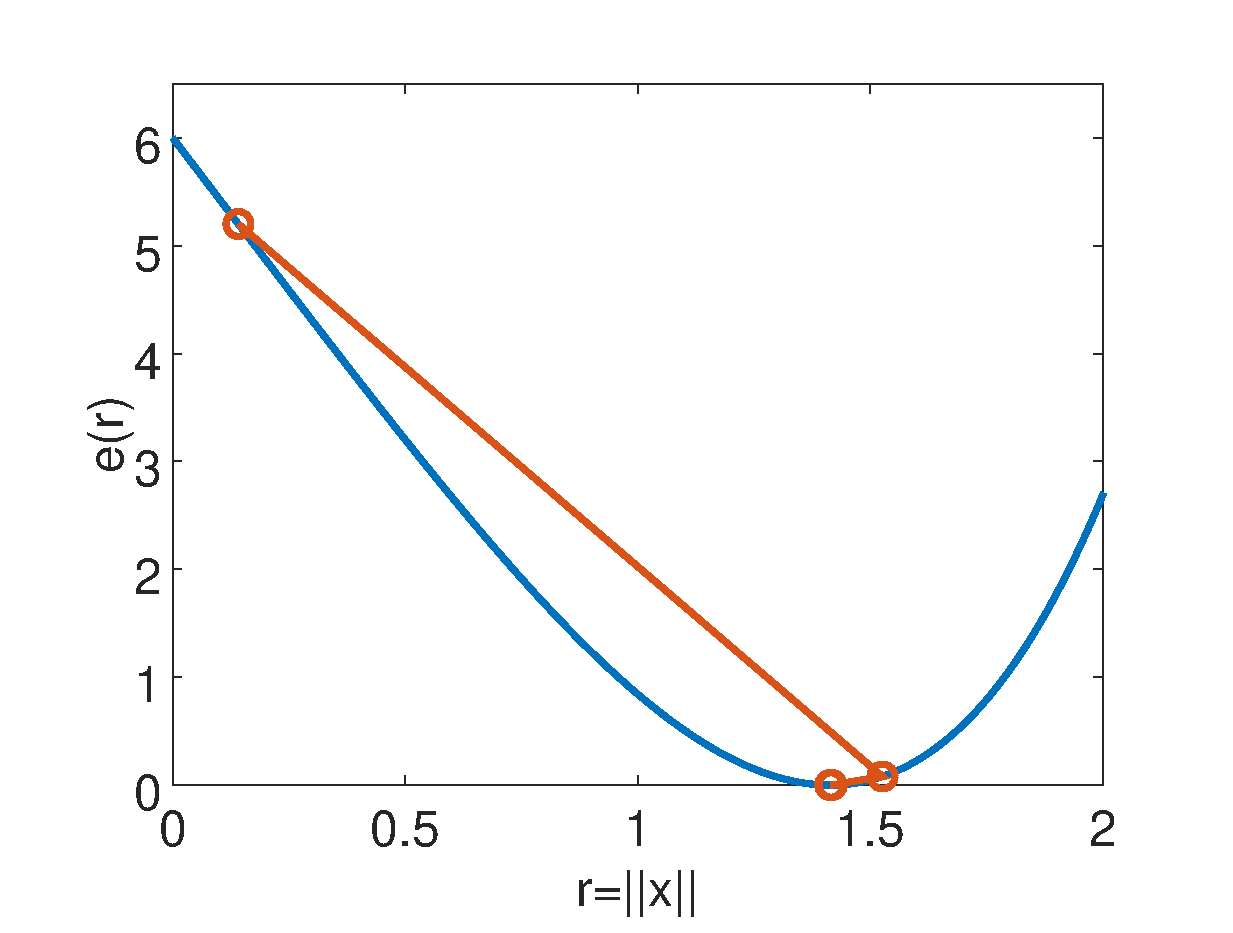
\includegraphics[width=0.98\textwidth]{chapters/minimization-fx/mfiles/fx1/plotfx.eps}
         \caption{Curva $e(\VECTOR{x})$ na direção $(1,1)$.}
         \label{fig:ex:minfxbCfxb:b}
     \end{subfigure}
        \caption{Resposta gráfica do Exemplo \ref{ex:minfxbCfxb}. }
        \label{fig:ex:minfxbCfxb}
\end{figure}


\begin{SolutionT}[Relativa ao Exemplo \ref{ex:minfxbCfxb}:]
\label{ex:minfxbCfxb:sol2}
É interessante resaltar que obteremos um erro,
se tentamos iniciar a busca iterativa desde a posição  $\VECTOR{x}_0=[0~0]^{\transpose}$
com pendente $\frac{\partial e(\VECTOR{x}_0)}{\partial \VECTOR{x} }=[-4~-4]^{\transpose}$,
pois a matriz $\MATRIX{J}(\VECTOR{x}_0)^{\transpose}\MATRIX{C} \MATRIX{J}(\VECTOR{x}_0)$
não tem inversa.
\end{SolutionT}


\begin{example}[Quando existe um
$\VECTOR{\hat{x}}$ que cumpre que $\VECTOR{f}(\VECTOR{\hat{x}}) \neq \VECTOR{b}$:]
\label{ex:minfxbCfxb2}
Conhecida uma função $\VECTOR{f}(\VECTOR{x}) : \mathbb{R}^{2} \rightarrow \mathbb{R}^{3}$
é um ponto $\VECTOR{b}$ que presumimos que existe no contradominio $\VECTOR{f}(\VECTOR{x})$,
achar o valor $\VECTOR{\hat{x}}$ que minimize $||\VECTOR{f}(\VECTOR{x})-\VECTOR{b}||_{\MATRIX{C}}^2$;
sabendo que:
\begin{equation}
\VECTOR{b}=\begin{bmatrix}
1\\
1\\
1.5
\end{bmatrix},
\qquad 
\VECTOR{f}(\VECTOR{x})=\begin{bmatrix}
x_1^2\\
x_2^2\\
x_1+x_2
\end{bmatrix}.
\end{equation}
Com todos estes dados e usando a Eq. (\ref{eq:minfxbCfxb1}),
obtemos a superfície $e(\VECTOR{x})$ como mostra a Figura \ref{fig:ex:minfxbCfxb2:a},
na qual observamos que esta nunca atinge o valor zero.
Podemos ver uma resposta para este exemplo na Solução \ref{ex:minfxbCfxb2:sol1}.
\end{example}

\begin{SolutionT}[Relativa ao Exemplo \ref{ex:minfxbCfxb2}:]
\label{ex:minfxbCfxb2:sol1}
Este problema pode ser resolvido de forma similar ao Exemplo \ref{ex:minfxbCfxb},
usando os dados da Eq. (\ref{eq:lab:ex2fx}).
Assim, se escolhemos o ponto inicial $\VECTOR{x}_0=[0.1~0.1]^{\transpose}$ 
e usamos iterativamente a Eq. (\ref{eq:minfxbCfxb2}) obtemos os valores 
de $\VECTOR{x}_k$ e $e(\VECTOR{x}_k)$, como mostra a Tabela \ref{table:ex:minfxbCfxb2}.
A aproximação iterativa é feita ate atingir $\VECTOR{x}_k \approx \VECTOR{x}_{k-1}$,
onde concluimos que a resposta é $\VECTOR{\hat{x}}\approx \VECTOR{x}_5 =[0.90856\quad 0.90856]^{\transpose}$
com um erro $e(\VECTOR{\hat{x}})=0.16148$; é dizer, não existe $\VECTOR{f}(\VECTOR{\hat{x}})$
que seja igual a $\VECTOR{b}$, só podemos achar um vetor $\VECTOR{\hat{x}}$ 
que provoque um valor com mínimo erro, com pendente 
$\frac{\partial e(\VECTOR{\hat{x}})}{\partial \VECTOR{x} }=[-9.7332~10^{-6}\quad -9.7332~{10}^{-6}]^{\transpose}$
e um
\begin{equation}
\MATRIX{J}(\VECTOR{\hat{x}})=
\begin{bmatrix}
1.81712 & 0.0\\ 
0.0     & 1.81712\\
1       & 1
\end{bmatrix}.
\end{equation}
Todo este processo pode ser visto de forma gráfica na Figura \ref{fig:ex:minfxbCfxb2:b}.
\end{SolutionT}

\begin{table}[h!]
\centering
\begin{tabular}{|l|l|l|l|l|l|l|}
\hline
$k$ & 0 & 1 & 2 & 3 & 4 & 5 \\ \hline
$\VECTOR{x}_k$ & 0.10000   & 0.83431   & 0.90507   & 0.90833   & 0.90855   & 0.90856 \\ 
~              & 0.10000   & 0.83431   & 0.90507   & 0.90833   & 0.90855   & 0.90856 \\ \hline
$||\VECTOR{x}_k||$ & 0.14142   & 1.17989   & 1.27996   & 1.28457   & 1.28488   & 1.28490 \\ \hline
$e(\VECTOR{x}_k)$ & 3.65020  & 0.21317  & 0.16160  & 0.16148  & 0.16148  & 0.16148 \\ \hline
\end{tabular}
\caption{Resposta iterativa do Exemplo \ref{ex:minfxbCfxb2}.}
\label{table:ex:minfxbCfxb2}
\end{table}
\begin{figure}[h!]
     \centering
     \begin{subfigure}[b]{0.49\textwidth}
         \centering
         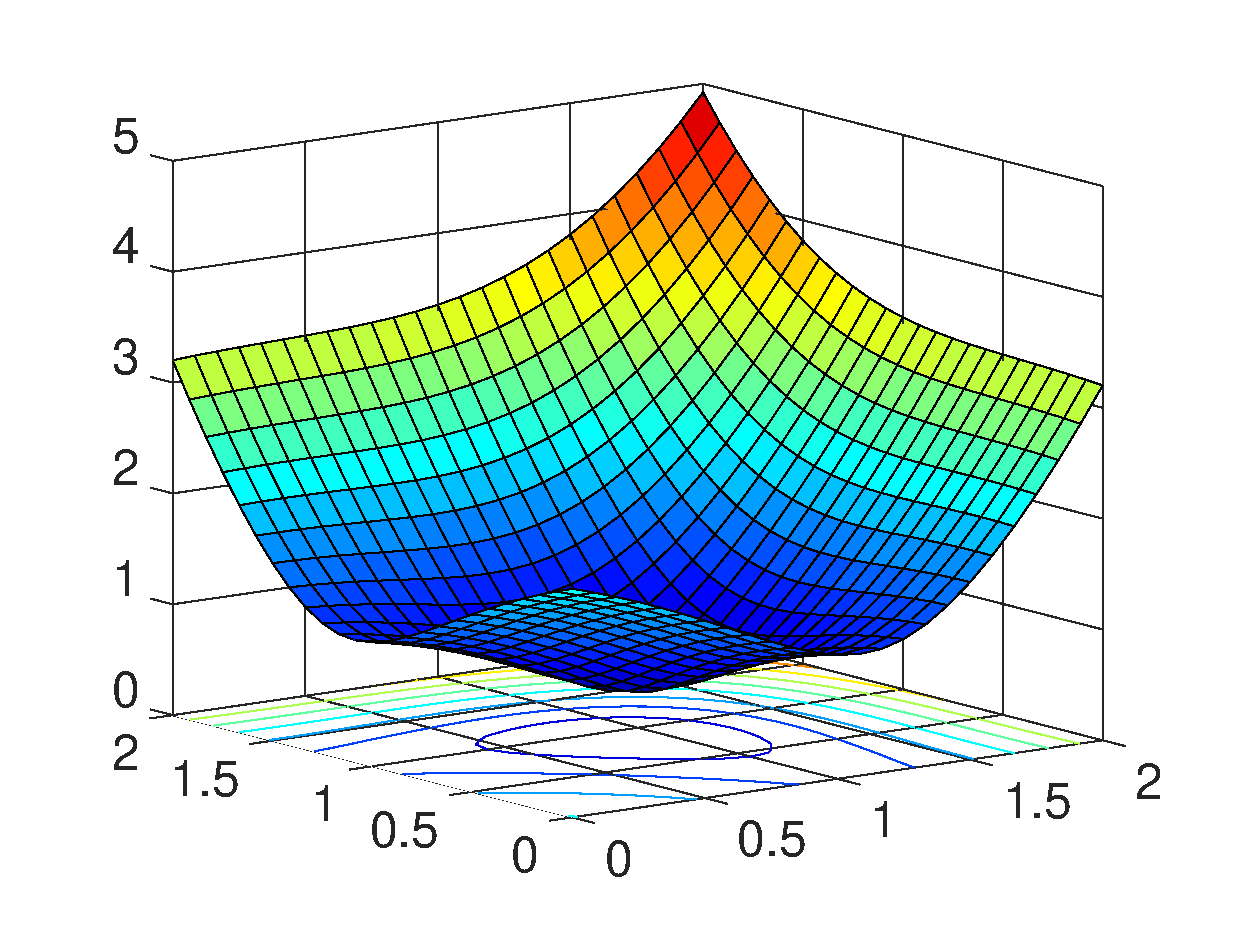
\includegraphics[width=0.98\textwidth]{chapters/minimization-fx/mfiles/fx1/surfcfx2.eps}
         \caption{Superfície $e(\VECTOR{x})$. }
         \label{fig:ex:minfxbCfxb2:a}
     \end{subfigure}
     \hfill
     \begin{subfigure}[b]{0.49\textwidth}
         \centering
         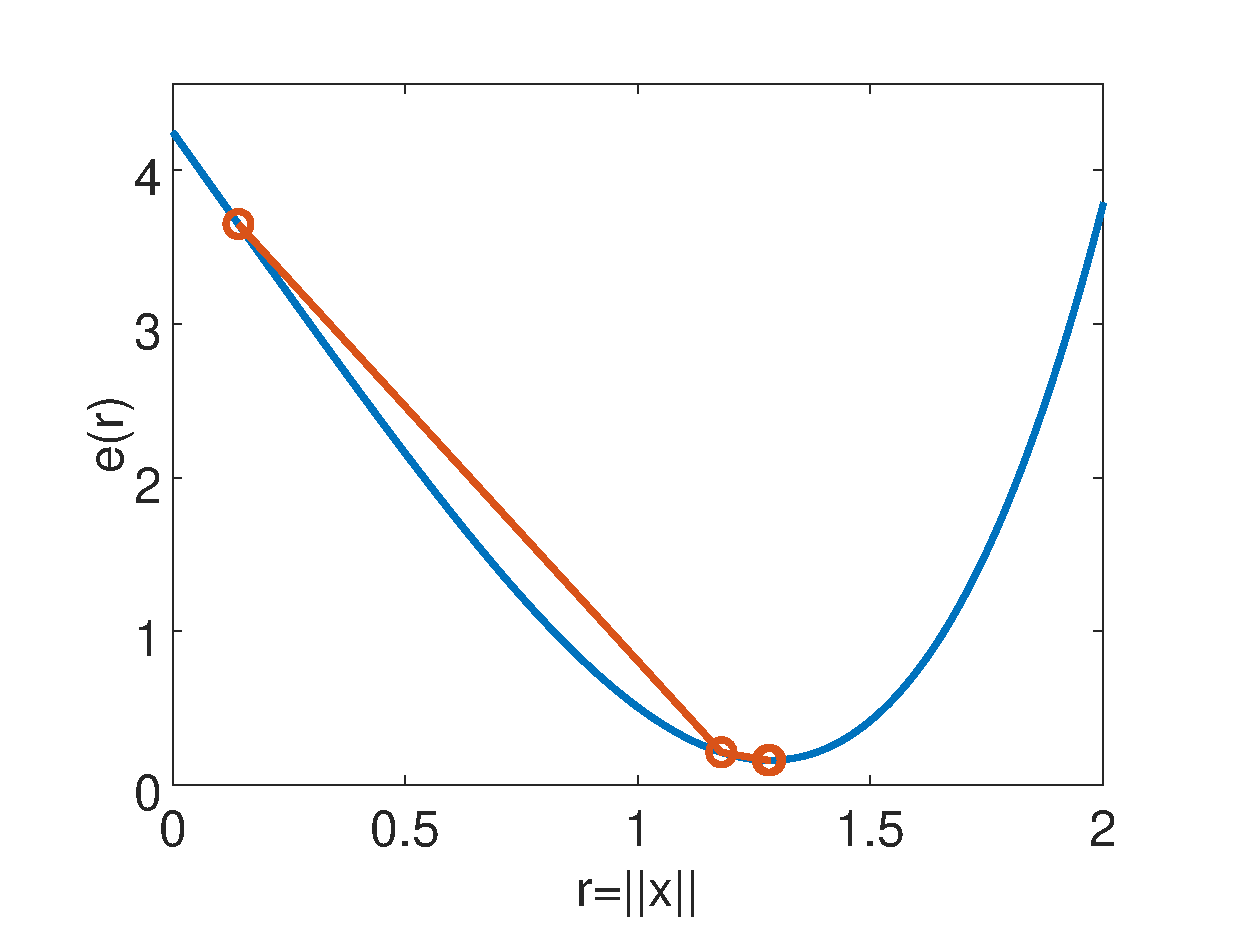
\includegraphics[width=0.98\textwidth]{chapters/minimization-fx/mfiles/fx1/plotfx2.eps}
         \caption{Curva $e(\VECTOR{x})$ na direção $(1,1)$.}
         \label{fig:ex:minfxbCfxb2:b}
     \end{subfigure}
        \caption{Resposta gráfica do Exemplo \ref{ex:minfxbCfxb2}. }
        \label{fig:ex:minfxbCfxb2}
\end{figure}


\begin{example}[Quando existem muitos mínimos locais e um
$\VECTOR{\hat{x}}$ que cumpre que $\VECTOR{f}(\VECTOR{\hat{x}}) \approx \VECTOR{b}$:]
\label{ex:minfxbCfxb3}
Conhecida uma função $\VECTOR{f}(\VECTOR{x}) : \mathbb{R}^{2} \rightarrow \mathbb{R}^{3}$
é um ponto $\VECTOR{b}$ do contradomínio de $\VECTOR{f}(\VECTOR{x})$,
achar o valor $\VECTOR{\hat{x}}$ que minimize $||\VECTOR{f}(\VECTOR{x})-\VECTOR{b}||_{\MATRIX{C}}^2$;
sabendo que:
\begin{equation}
\VECTOR{b}=\begin{bmatrix}
1\\
1\\
2
\end{bmatrix},
\qquad 
\VECTOR{f}(\VECTOR{x})=\begin{bmatrix}
sin(\frac{x_1 5 \pi}{2})\\
sin(\frac{x_2 5 \pi}{2})\\
x_1+x_2
\end{bmatrix}.
\end{equation}
Consequentemente podemos deduzir e escolher que, 
\begin{equation}\label{eq:lab:ex2fx3}
\MATRIX{J}(\VECTOR{x})=\begin{bmatrix}
\frac{5 \pi}{2}cos(\frac{x_1 5 \pi}{2}) & 0\\
0 & \frac{5 \pi}{2}cos(\frac{x_2 5 \pi}{2}) \\
1 & 1
\end{bmatrix},
\qquad
\MATRIX{C}=\begin{bmatrix}
1 & 0 & 0\\
0 & 1 & 0\\
0 & 0 & 1
\end{bmatrix}.
\end{equation}
Com todos estes dados e usando a Eq. (\ref{eq:minfxbCfxb1}),
obtemos a superfície $e(\VECTOR{x})$ como mostra a Figura \ref{fig:ex:minfxbCfxb3:a}.
Podemos ver as respostas a este exemplo na Solução \ref{ex:minfxbCfxb3:sol1} e \ref{ex:minfxbCfxb3:sol2}.
\end{example}

\begin{SolutionT}[Relativa ao Exemplo \ref{ex:minfxbCfxb3}:]
\label{ex:minfxbCfxb3:sol1}
Se escolhemos o ponto inicial $\VECTOR{x}_0=[\frac{11.0999}{5}$ $\frac{11.0999}{5}]^{\transpose}$,
com pendente\footnote{O cálculo da
pendente de $e(\VECTOR{\hat{x}})$ pode ser visto no Teorema \ref{theo:derfxbCfxb0}.} 
$\frac{\partial e(\VECTOR{x}_0)}{\partial \VECTOR{x} }=[4.2318~10^{-4}\quad 4.2318~10^{-4}]^{\transpose}$ e 
usamos iterativamente a Eq. (\ref{eq:minfxbCfxb2}), obtemos os valores 
de $\VECTOR{x}_k$ e $e(\VECTOR{x}_k)$, como mostra a Tabela \ref{table:ex:minfxbCfxb3},
onde se asume o final do processo iterativo quando $\VECTOR{x}_k \approx \VECTOR{x}_{k-1}$.
Assim, a aproximação iterativa conclui na resposta $\VECTOR{\hat{x}}\approx \VECTOR{x}_{7} =[1.7076\quad 1.7076]^{\transpose}$
com um erro $e(\VECTOR{\hat{x}})=2.1298$, uma pendente
$\frac{\partial e(\VECTOR{\hat{x}})}{\partial \VECTOR{x} }=[0.20251\quad 0.20251]^{\transpose}$
e um
\begin{equation}
\MATRIX{J}(\VECTOR{\hat{x}})=
\begin{bmatrix}
5.21306 & 0.0\\ 
0.0     & 5.21306\\
1       & 1
\end{bmatrix};
\end{equation}
este processo pode ser visto de forma gráfica na Figura \ref{fig:ex:minfxbCfxb3:b}.

É interesante resaltar que o ponto $\VECTOR{x}_0$ é muito próximo a um máximo local de 
$e(\VECTOR{x})$, e o uso iterativo da Eq. (\ref{eq:minfxbCfxb2}) 
provoca o afastamento deste ponto, mesmo que a princípio os passos sejam pequenos;
por outro lado, a busca iterativa converge e finaliza em $\VECTOR{x}_7$ um mínimo local 
de $e(\VECTOR{x})$.

\end{SolutionT}

\begin{table}[h!]
\centering
\begin{tabular}{|l|l|l|l|l|l|l|l|l|}
\hline
$k$ & 0 & 1 & 2 & 3 & 4 & 5 & 6 & 7\\ \hline
$\VECTOR{x}_k$ & 2.2200   & 2.2199   & 2.2178   & 2.1385   & 1.5400   & 1.7184   & 1.6974   & 1.7076 \\ 
~              & 2.2200   & 2.2199   & 2.2178   & 2.1385   & 1.5400   & 1.7184   & 1.6974   & 1.7076 \\ \hline
$||\VECTOR{x}_k||$ & 3.1396   & 3.1394   & 3.1364   & 3.0243   & 2.1779   & 2.4302   & 2.4005   & 2.4149 \\ \hline
$e(\VECTOR{x}_k)$ & 13.8554  & 13.8554  & 13.8543  & 12.2971   & 5.3932   & 2.1432   & 2.1346   & 2.1298 \\ \hline
\end{tabular}
\caption{Resposta iterativa do Exemplo \ref{ex:minfxbCfxb3}.}
\label{table:ex:minfxbCfxb3}
\end{table}
\begin{figure}[h!]
     \centering
     \begin{subfigure}[b]{0.49\textwidth}
         \centering
         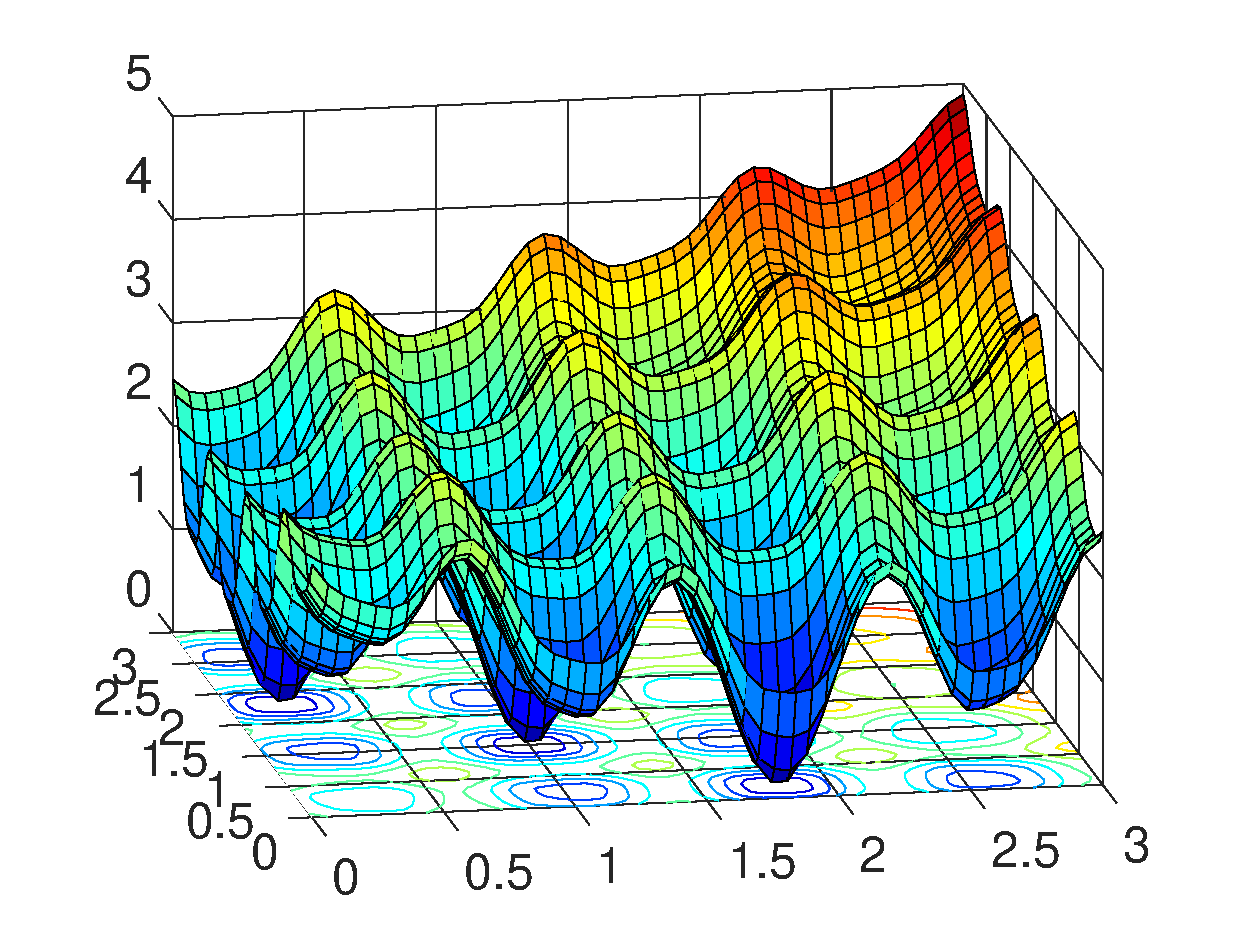
\includegraphics[width=0.98\textwidth]{chapters/minimization-fx/mfiles/fx3/surfcfx3.eps}
         \caption{Superfície $e(\VECTOR{x})$. }
         \label{fig:ex:minfxbCfxb3:a}
     \end{subfigure}
     \hfill
     \begin{subfigure}[b]{0.49\textwidth}
         \centering
         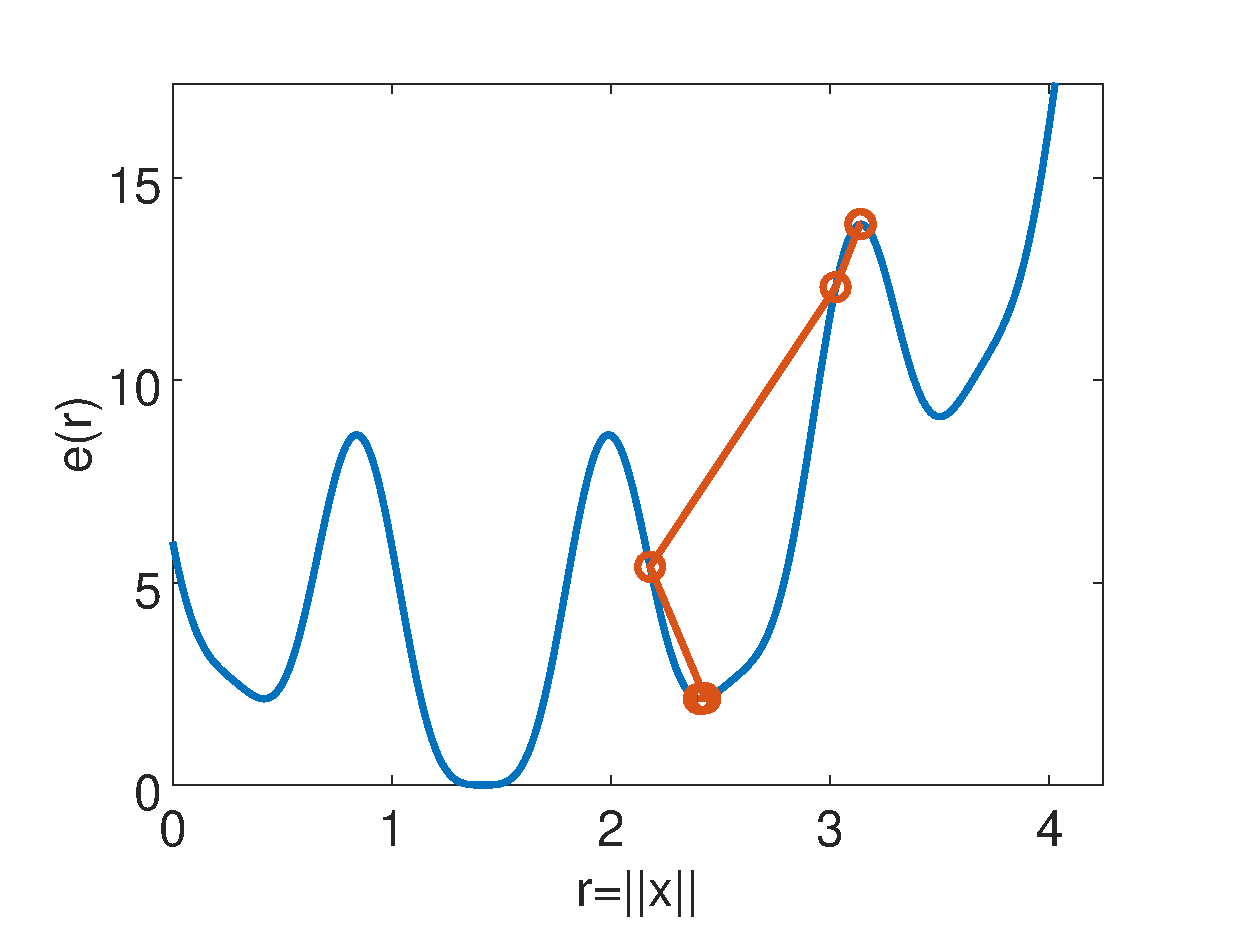
\includegraphics[width=0.98\textwidth]{chapters/minimization-fx/mfiles/fx3/plotfx3.eps}
         \caption{Curva $e(\VECTOR{x})$ na direção $(1,1)$.}
         \label{fig:ex:minfxbCfxb3:b}
     \end{subfigure}
        \caption{Resposta gráfica do Exemplo \ref{ex:minfxbCfxb3}. }
        \label{fig:ex:minfxbCfxb3}
\end{figure}

\begin{SolutionT}[Relativa ao Exemplo \ref{ex:minfxbCfxb3}:]
\label{ex:minfxbCfxb3:sol2}
Se escolhemos o ponto inicial $\VECTOR{x}_0=[\frac{7.032993}{5}$ $\frac{7.032993}{5}]^{\transpose}$,
com pendente\footnote{O cálculo da
pendente de $e(\VECTOR{\hat{x}})$ pode ser visto no Teorema \ref{theo:derfxbCfxb0}.} 
$\frac{\partial e(\VECTOR{x}_0)}{\partial \VECTOR{x} }=[7.6342~10^{-5}\quad 7.6342~10^{-5}]^{\transpose}$ e 
usamos iterativamente a Eq. (\ref{eq:minfxbCfxb2}), obtemos os valores 
de $\VECTOR{x}_k$ e $e(\VECTOR{x}_k)$, como mostra a Tabela \ref{table:ex:minfxbCfxb4},
onde se asume o final do processo iterativo quando $\VECTOR{x}_k \approx \VECTOR{x}_{k-1}$.
Assim, a aproximação iterativa conclui na resposta $\VECTOR{\hat{x}}\approx \VECTOR{x}_{7} =[0.99056\quad 0.99056]^{\transpose}$,
com um erro $e(\VECTOR{\hat{x}})=3.7152~10^{-4}$, uma pendente
$\frac{\partial e(\VECTOR{\hat{x}})}{\partial \VECTOR{x} }=[-0.040955\quad -0.040955]^{\transpose}$
e um
\begin{equation}
\MATRIX{J}(\VECTOR{\hat{x}})=
\begin{bmatrix}
0.58175 & 0.0\\ 
0.0     & 0.58175\\
1       & 1
\end{bmatrix};
\end{equation}
este processo pode ser visto de forma gráfica na Figura \ref{fig:ex:minfxbCfxb4:b}.

De forma similar ao Exemplo \ref{ex:minfxbCfxb3:sol1}, observamos 
que o ponto $\VECTOR{x}_0$ é muito próximo a um máximo local de 
$e(\VECTOR{x})$, e o uso iterativo da Eq. (\ref{eq:minfxbCfxb2}) 
provoca o afastamento deste ponto, mesmo que a princípio os passos sejam pequenos;
por outro lado, a busca iterativa converge e finaliza em $\VECTOR{x}_7$ um mínimo global
de $e(\VECTOR{x})$.
\end{SolutionT}


\begin{table}[h!]
\centering
\begin{tabular}{|l|l|l|l|l|l|l|l|l|}
\hline
$k$ & 0 & 1 & 2 & 3 & 4 & 5 & 6 & 7\\ \hline
$\VECTOR{x}_k$ & 1.40660   & 1.40658   & 1.40558   & 1.34728   & 0.78432   & 0.93066   & 0.96985   & 0.99056 \\ 
~              & 1.40660   & 1.40658   & 1.40558   & 1.34728   & 0.78432   & 0.93066   & 0.96985   & 0.99056 \\ \hline
$||\VECTOR{x}_k||$ & 1.9892   & 1.9892   & 1.9878   & 1.9053   & 1.1092   & 1.3162   & 1.3716   & 1.4009 \\ \hline
$e(\VECTOR{x}_k)$ & 8.6506  & 8.6506  & 8.6503  & 7.8206  & 2.7076  & 6.109e-2 &  5.192e-3  & 3.715e-4 \\ \hline
\end{tabular}
\caption{Resposta iterativa do Exemplo \ref{ex:minfxbCfxb3}.}
\label{table:ex:minfxbCfxb4}
\end{table}

     \begin{figure}[!h]
         \centering
         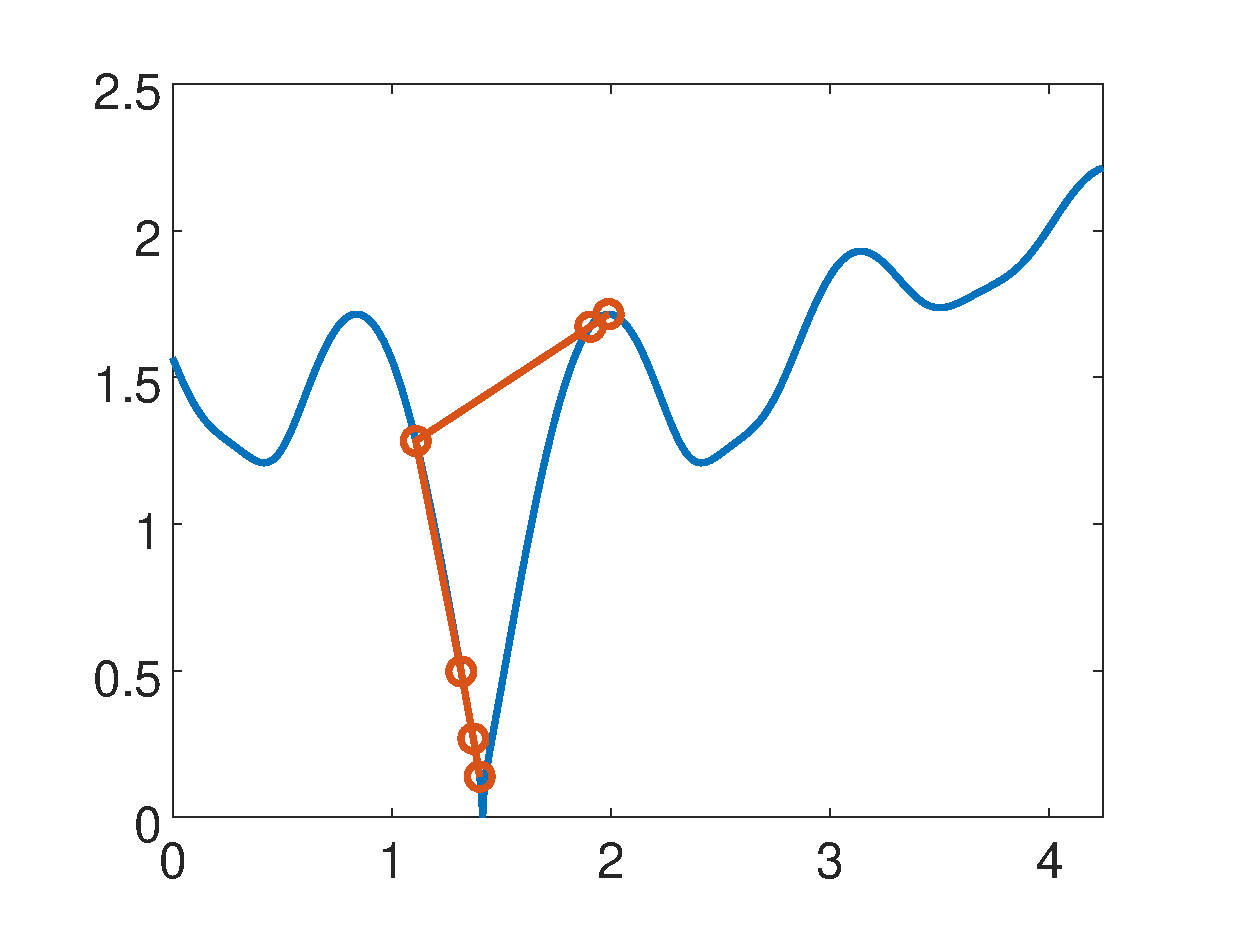
\includegraphics[width=0.5\textwidth]{chapters/minimization-fx/mfiles/fx3/plotfx4.eps}
         \caption{Curva $e(\VECTOR{x})$ na direção $(1,1)$.}
         \label{fig:ex:minfxbCfxb4:b}
     \end{figure}


